\chapter{EPUB Document Standard}
\label{ch:EPUB Document Standard}

\section{Requirements}

One requirement of the new standard is that incorporates a way to switch between three versions, them being:

\begin{itemize}
	\item Blind
	\item Visually Impaired
	\item Normal sighted
\end{itemize}

Switching between three versions should be simple and visible. It should not be hidden behind menus and settings and must be part of the document itself. A document of the standard must conform to EPUB 3 and not rely on external programs to switch between the versions.

The specifications of each version will be compared with each important component of a document.


\subsection{Switching between versions}

Initially the intent was to find one new standard so that EPUB documents can be accessible. Unfortunately, creating a single standard was not possibles since not all EPUB readers support all EPUB 3 features yet.

\subsubsection{JavaScript}
JavaScript is used to make websites interactive, so it was the logical option to dynamically change the versions. The coding was also quite simple and only involved replacing a single line in the CSS file with programming. This was easy to do in JavaScript, and testing the individual XHTML files in the EPUB showed that it was successful. 

Shown in figure \ref{fig:jsStyleCss} are the contents of the file style.css. All it does is import the CSS rules of different CSS file. The methods \lstinline|selectVisible()|, \lstinline|selectImpaired()| and \lstinline|selectBlind()| in script.js all function in the same way. To remember the version chosen, local and session storage are used. Both of them are used by web browsers to remember settings of websites. Session storage is saved until the web browser is closed, while local storage remains even after the browser has been closed. The methods check if local storage is available. If it is then the method attempts to get the item \lstinline|accessibleEPUBcurrentCSS|. If it does not exist, then it is created. This item is then set with the same import line in figure \ref{fig:jsStyleCss}, only with a different CSS filename for each version. If local storage is not available the same process is repeated with session storage. Local storage is preferable to session storage as changes are kept even after the program has been exited. This is not the case with session storage so the user has to set version again at the start of the program. Afterwards the method \lstinline|loadCSS()| is called which deletes the CSS rule of a XHTML file and adds the rule set by the earlier methods.

The content of the XHTML file responsible for the switching mechanism, VersionChanger.xhtml, is shown in figure \ref{fig:js_switch}. It is important that both style.css and script.js are referred to, or the switching mechanism would be unsuccessful. In the body of the XHTML document, the method \lstinline{storageCSS()} is called whenever the XHTML file is loaded. This happens if the page is turned to that file. This method checks if local and then session storage are available. If either one is avaiable then it sets the item in the storage and calls \lstinline{loadCSS()}.

\begin{figure}
	
	\begin{lstlisting}
	@import url("../Styles/visible.css");
	\end{lstlisting}
	\caption{Contents of style.css}
	\label{fig:jsStyleCss}
\end{figure}

\begin{figure}
	
	\begin{lstlisting}
	<head>
	<title></title>
	<link rel="stylesheet" href="../Styles/style.css"/>
	<script src="../Misc/script.js"></script>
	</head>
	
	<body epub:type="frontmatter" onload="storageCSS();">
	<a id="a1" href="#a1" onclick="selectVisible();">Normal</a>
	<a id="a2" href="#a2" onclick="selectImpaired();">Visually impaired</a>
	<a id="a3" href="#a3" onclick="selectBlind();">Blind</a>
	</body>
	\end{lstlisting}
	\caption{The links in the JavaScript version}
	\label{fig:js_switch}
\end{figure}

There are some issues with the JavaScript version changer. If the software or hardware reader does not support temporary storage, the EPUB is always displayed in its default appearance. Due to this, switching with JavaScript is not a reliable option. As mentioned in chapter \ref{ch:Introduction}, JavaScript does not have to be supported by all EPUB readers. Nevertheless, the JavaScript implementation supports multiple XHTML files, because temporary storage is supported. For the same reason table of contents are also supported, as they are normally displayed in a separate file, named \lstinline|nav.xhtml|. 

\subsubsection{CSS}
The second method does not use JavaScript and uses some advanced features of CSS, introduced in CSS 3. This mainly refers to CSS selectors. Selectors allow HTML documents to have limited interactive capabilities, such as changing the appearance of a clicked element\footnote{https://www.w3schools.com/cssref/css\_selectors.asp} \cite{cssSelectors}.

Before showing how the selectors work, the format of the content file should be discussed. It is shown in figure~\ref{fig:css_switch}. Unlike the JavaScript version, the links are in the same XHTML file and are shown at the beginning of the EPUB file. In the JavaScript version, the links are on a separate page.


\begin{figure}
	
	\begin{lstlisting}
	<body>
	<a class="versionChanger" id="a1" href="#visible">Normal</a>
	<a class="versionChanger" id="a2" href="#impaired">Visually impaired</a>
	<a class="versionChanger" id="a3" href="#blind">Blind</a>
	
	<div style="padding:none" id="impaired" class="impaired">
	...
	</div>
	<div id="blind" class="blind">
	...
	</div>
	<div id="visible" class="visible">
	...
	</div>
	</body>
	\end{lstlisting}
	\caption{The links and divs in the CSS version}
	\label{fig:css_switch}
\end{figure}

The code shown in figure~\ref{fig:css_selector} is responsible for the switching mechanism. At first only the visible version can be seen and the other two are hidden. The versions appear with the \lstinline|:target| selector, which affects the appearance of the element if it was a target of a link(\lstinline|<a> element|). If another link was clicked, then the current version becomes hidden again. However, the visible version would not become hidden, and this was a major problem. CSS selectors have limited capabilities compared to JavaScript, because they were intended to complement and not replace each other. After testing various CSS selectors, the \lstinline|~| selector delivered the desired results. \lstinline|~| allows every element on the right hand side to be selected if it preceded by a left hand side element. So in the case of \lstinline|.impaired:target ~ .visible|, once the impaired link has been clicked, the visible sections becomes hidden.

\begin{figure}
	
	\begin{lstlisting}
	.visible {
	display:inline; 
	}
	
	.impaired:target ~ .visible {
	display:none; 
	}
	
	.blind:target ~ .visible {
	display:none; 
	}
	
	.impaired {
	display:none; 
	}
	
	.blind {
	display:none; 
	}
	
	.impaired:target{
	display:inline; 
	}
	
	.blind:target{
	display:inline; 
	}
	\end{lstlisting}
	\caption{The CSS selectors responsible for the dynamic version switching}
	\label{fig:css_selector}
\end{figure}

\subsection{Text}

The blind version does not need any special requirements for text formatting, and its appearance will be identical to the normal version. The text size could be made much smaller, but leaving it at a standard size will allow other people to also read the text, such as for proofreading of the blind version.

The visually impaired version needs to use sans-serif fonts, as seen in figure \ref{fig:sansSerif}, instead of serif fonts, as it easier to read and identify individual characters \cite{pdfBarrierefrei}. Furthermore, the font should be larger than the normal version and the font size should be adaptable by the user. It is important that both superscripts and subscripts should be as large as the regular text.

\begin{figure}
	
	\begin{center}
		
\includegraphics[width=\linewidth/2]{figures/sansSerif.jpg}
	\end{center}

	
	\caption{Comparison of serif(left) and sans serif(right) fonts
		\\Source: https://cdncms.fonts.net/images/6bff0c2cdbbcca14/A.SerifSansPrint.jpg}
	\label{fig:sansSerif}
\end{figure}

The font of the normal version can be any font, but for this standard a serif font was chosen. Most importantly, the text should not go beyond the edge of the screen so that horizontal scrolling is not required. All normal text in the document will be between \lstinline|<p>| and \lstinline|</p>| tags. A comparison of the visually impaired and normal version can be seen in figures \ref{fig:viText} and \ref{fig:nText}. 

\begin{figure}
	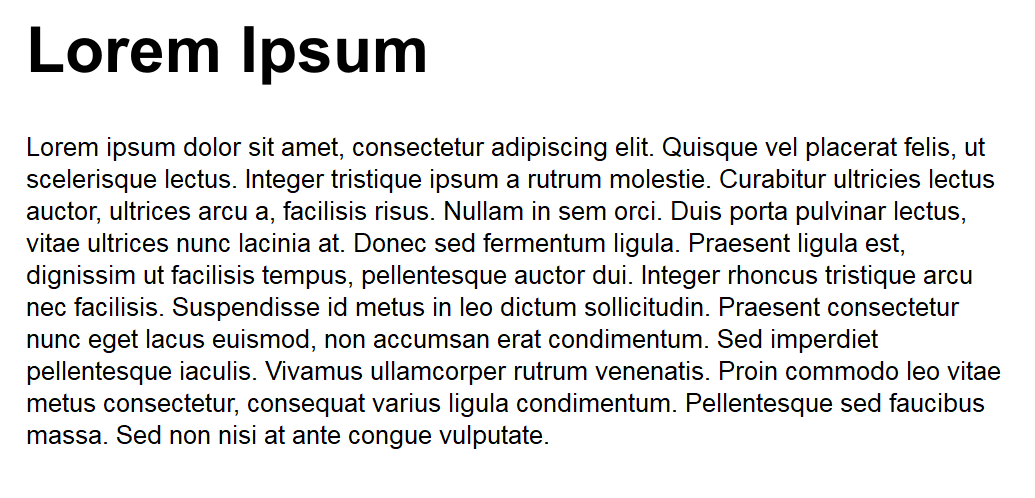
\includegraphics[width=\linewidth]{figures/VItext.png}	
	\caption{Text of the visually impaired version}
	\label{fig:viText}
\end{figure}

\begin{figure}
	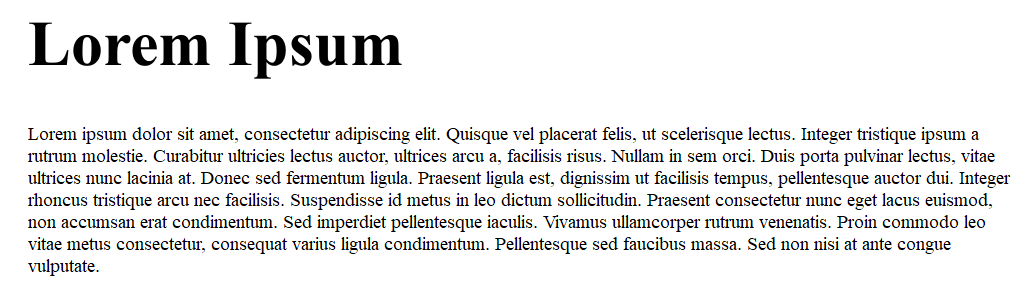
\includegraphics[width=\linewidth]{figures/Ntext.png}	
	\caption{Text of the normal version}
	\label{fig:nText}
\end{figure}

\subsection{Images}

All images need to have alternative text to describe them and preferably have a title given to them. This will help blind users as the screen reader will read out both of them. Usually the alternative text will be set as a property and the screen reader will have to identify the image. However, there was an issue. In some programs the screen reader does not read out the alternative text, so a different way had to be found to display it. The image will be part of a figure element of HTML5, shown in figure~\ref{fig:image_code}. A figure can also contain a caption, which will be identified by the screen reader as such, seen in  figure~\ref{fig:image_viimp} Furthermore, the alternative text will be inserted as a paragraph with the \lstinline|<p>| element. It will remain invisible in normal and visually impaired mode, but will appear as normal text in blind mode. The text should be surrounded by specific tags, like <Image> or <Graph> shown in figure~\ref{fig:image_blind}. It also has the CSS class "transparent", which only appears in blind mode.

Images in visually impaired and normal mode will be displayed normally, but the image, caption and figure will all have a maximum length of 100\% of the screen size.

\begin{figure}[H]
	\centering
	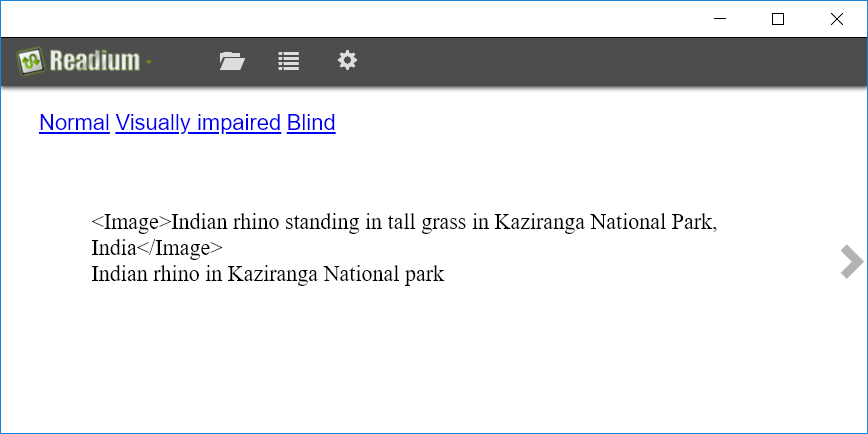
\includegraphics[width=\linewidth]{figures/ImageBl.PNG}
	\caption{Image in 'Blind' mode}
	\label{fig:image_blind}
\end{figure}

\begin{figure}[H]
	\centering
	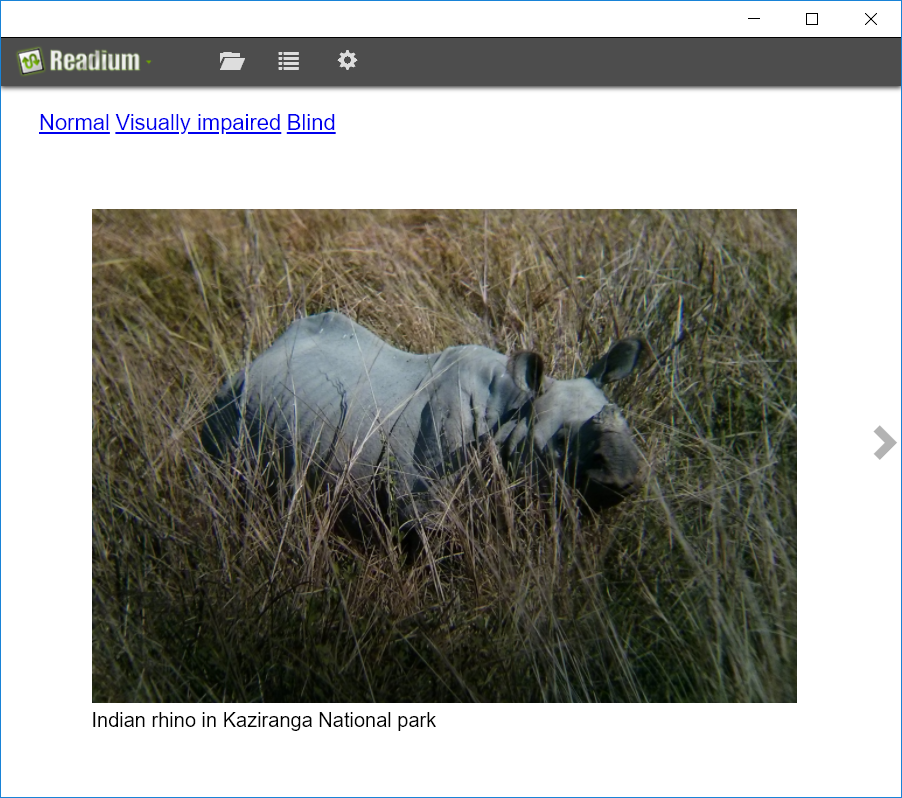
\includegraphics[width=\linewidth]{figures/ImageVi.PNG}
	\caption{Image in 'Visual impairment' mode}
	\label{fig:image_viimp}
\end{figure}



\begin{figure}[H]
	\lstset{language=HTML}
	\begin{lstlisting}
	<figure>
		<img title="KazirangaRhino" alt="Indian rhino standing in tall grass in Kaziranga National Park, India" src="..\Images\KazirangaRhino.png"/>
		<p class="transparent">
			&lt;Image&gt;Indian rhino standing in tall grass in Kaziranga National Park, India&lt;/Image&gt;
		</p>
		<figcaption> 
			Indian rhino in Kaziranga National park
		</figcaption>
	</figure>
	\end{lstlisting}
	\caption{Code of figure~\ref{fig:image_viimp} and \ref{fig:image_blind}}
	\label{fig:image_code}
\end{figure}

\subsection{Mathematical formulas}

Formulas should be stored in MathML. MathML is quite clunky and time consuming to write in, so a \LaTeX to MathML converter is used. % For the sample documents, a online converting tool was used. The input formula was the quadratic equation, which appeared in \ref{fig:quadEquaPng}.

\begin{figure}[H]
	\centering
	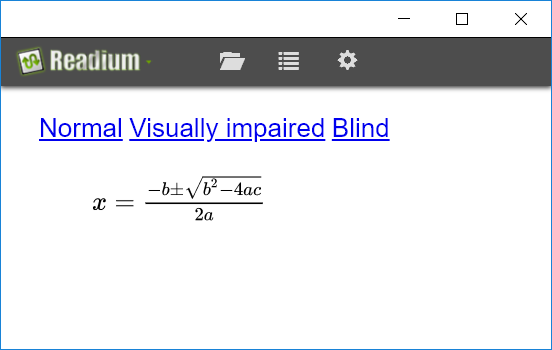
\includegraphics[width=\linewidth*2/3]{figures/EquationNo.PNG}
	\caption{Equation in 'Normal' mode}
	\label{fig:equation_normal}
\end{figure}
\vspace{-0.6cm}
\begin{figure}[H]
	\centering
	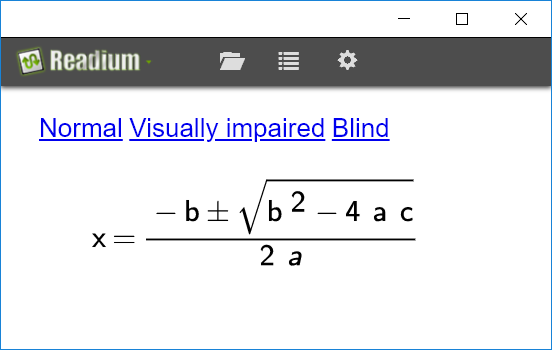
\includegraphics[width=\linewidth*2/3]{figures/EquationVi.PNG}
	\caption{Equation in 'Visual impairment' mode}
	\label{fig:equation_viimp}
\end{figure}



In the normal version the default display style is used, which uses a serif font and a combination of italicized and unitalicized letters, as shown in figure~\ref{fig:equation_normal}. Serif fonts are not suitable in the visually impaired version, so a sans serif had to be chosen. At first the font was changed in the CSS. This unfortunately resulted in the text not scaling properly, and therefore some characters were not properly spaced. The root symbol also wasn't displayed clearly. Instead the mstyle attribute of MathML had to be changed to sans serif which resulted in figure~\ref{fig:equation_viimp}. The mstyle attribute can not be changed in CSS, it has to be inserted into every math element.

\begin{figure}[H]
	\centering
	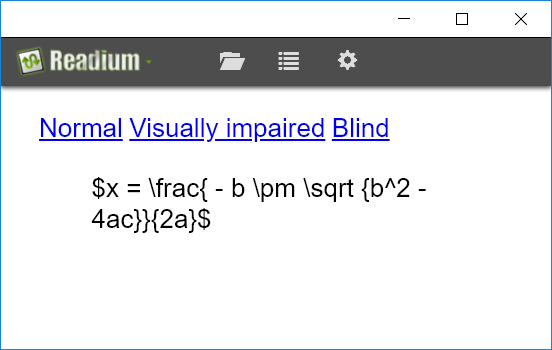
\includegraphics[width=\linewidth*2/3]{figures/EquationBl.PNG}
	\caption{Equation in 'Blind' mode}
	\label{fig:equation_blind}
\end{figure}

In the blind version, the text has to appear as \LaTeX code. Much like the alternative text for images, it will appear as a separate paragraph enclosed in \lstinline{<p>}  tags. To signify that it is code, it has to be surrounded by \$ signs, as shown in figure~\ref{fig:equation_blind}. The math element is in a \lstinline{<div>} with CSS class "math", which is hidden in the blind version.

\vspace{0.6cm}
\lstset{language=HTML}
\begin{lstlisting}
<figure>
<div role="math" class="math">
<math xmlns="http://www.w3.org/1998/Math/MathML" id="Formula" title="Quadratic Formula" alttext="{x=\frac{-b\pm\sqrt{b^2-4ac}}{2a}}">
<mstyle>
<semantics>

<mrow>
<mi>x</mi>
<mo>=</mo>
<mfrac>
<mrow>
<mrow>
<mo>-</mo>
<mi>b</mi>
</mrow>
<mo>%*±</mo>*)
<msqrt>
<mrow>
<msup>
<mi>b</mi>
<mn>2</mn>
</msup>
<mo>-</mo>
<mrow>
<mn>4</mn>
<mo></mo>
<mi>a</mi>
<mo></ mo>
<mi>c</mi>
</mrow>
</mrow>
</msqrt>
</mrow>
<mrow>
<mn>2</mn>
<mo></mo>
<mi>a</mi>
</mrow>
</mfrac>
</mrow> 

</semantics>
</mstyle>
</math>
</div>

<p class="transparent">
$x = \frac{ - b \pm \sqrt {b^2 - 4ac}}{2a}$
</p>

</figure>
\end{lstlisting}

\begin{figure}[H]

	
\caption{Code of figures \ref{fig:equation_normal} and \ref{fig:equation_blind}}
	\label{fig:math_code}
\end{figure}

\begin{figure}[H]
	\lstset{language=HTML}
	\begin{lstlisting}
		<mstyle scriptsizemultiplier="1" lspace="20%" rspace="20%" mathvariant="sans-serif">
	\end{lstlisting}
	\caption{Addition to the code shown in \ref{fig:math_code} for the visually impaired version to make the formula appear as sans serif and not in italics}
		\label{fig:math_vi_code}
\end{figure}


